\documentclass[12pt,  english, makeidx, a4paper, titlepage, oneside]{article}
\usepackage[english]{babel}
\usepackage[applemac]{inputenc}
\usepackage{fancyhdr}
\usepackage{makeidx}
\usepackage{titlesec}
\usepackage{listings} 
\newenvironment{listato}{\footnotesize}
                        {\normalsize }
\textwidth 19cm
\textheight 23cm
\topmargin -1.5cm
\oddsidemargin -1.5cm
\linespread{1.1}

\pagestyle{fancy}
\lhead{}
\chead{Module name}
\lfoot{}
\cfoot{}
\rfoot{}
\rhead{\thepage}

\usepackage{graphicx}
\usepackage{amsmath}
\usepackage{amsfonts}
\usepackage{amsthm}
\usepackage{amssymb}


\titleformat{\chapter}[display]
{\normalfont\Large\filcenter\sffamily}
{\titlerule[0.5pt]%
\vspace{1pt}
\titlerule
\vspace{1pc}
\LARGE\MakeUppercase{\chaptertitlename} \thechapter
}
{1pc}
{\titlerule
\vspace{1pc}
\Huge}

\makeindex

\begin{document}
\begin{titlepage}
\vspace{2cm}
\centerline{

\includegraphics[width=2cm]{./img/logopoli.eps}}  
\centerline{\LARGE Politecnico di Torino}
\bigskip
\centerline{\Large III Facolt\`a di Ingegneria}
\vspace{4cm}
\centerline{\Huge\sf NAND-2 inputs analysis}
\bigskip
\centerline{\Huge\bfseries\sf Integrated system technology}
\vspace{2cm}
\centerline{\Large GROUP: 15}
\vspace{2cm}
\centerline{\Large Francesco Lo Presti\\Simone Massimino\\Giuseppe Serafini}
\vspace{2cm}
\centerline{\Large \today}
\end{titlepage}

\tableofcontents

\newpage

\lstset{language=Matlab}

\newpage
\section{Introduction}
The aim of this project is to create a parametrical model to describe the behaviour of the basic components used to realize arithmetical circuits, the half adder and the full adder. In the Theoretical analysis is discussed the general description of both components above mentioned and then the calculation of power consumption, occupied area and timing. The calculations have been executed transforming the logic gates inside the structure in NAND gates; this is a choice made in order to simplify calculations of power and timing. In the Octave implementation is shown the Matlab code used to realize the models. Moreover, two tables, which list the legend of the parameters, have been created in order to help the reader during the reading of this document. The last section concerns the results for each analysis indicated above. The used technological parameters refer to Bulk Technology HP 2009.

\section{Theoretical analysis}
\subsection{Half Adder}
The half adder circuit is shown in figure \ref{half_adder}:
\begin{figure}[h]
	\caption{Half adder}
	\includegraphics[width=5cm]{img/half_adder.png}
	\centering
	\label{half_adder}
\end{figure}
As shown in the figure, the half adder generates two outputs starting from two input bits. The S bit represents the sum bit, and has the logic function:
\begin{equation}
S = A \oplus B
\end{equation}
The C bit represents the carry bit, and the logic function is:
\begin{equation}
C = AB
\end{equation}
\subsubsection{Area}\label{area_ha}
As said in chapter \ref{intro}, all logic gates will be considered as NAND gates. The XOR gate in NAND technology becomes as shown in figure \ref{xor_to_nand} \cite{rif1}.
\begin{figure}[h]
	\caption{XOR gate realized with NAND gates}
	\includegraphics{img/xor_to_nand.png}
	\centering
	\label{xor_to_nand}
\end{figure}
The area occupied by the XOR gate in NAND technology is four times the area occupied by a single NAND gate; in the calculations, the area override due to interconnections has been taken into account. The CMOS structure of the NAND gate is shown in figure \ref{nand_gate_MOS}.
\begin{figure}
	\caption{NAND gate in CMOS technology}
	\includegraphics{img/nand_gate_transistor.png}
	\centering
	\label{nand_gate_MOS}
\end{figure}
By theory, the area of a single NAND gate is computed as:
\begin{equation}
area_{NAND} = 2\cdot (W_n + W_p)\cdot (1 + override)\cdot L
\end{equation}
\begin{itemize}
	\item $W_n$ is the channel width for nMOS;
	\item $W_p$ is the channel width for pMOS;
	\item $L = L_{eff} + 2L_{s,d}$ is the total channel length; $L_{eff}$ is the effective gate length, while $L_{s,d}$ is the source length, equal to the drain length, hence the factor 2;
	\item $override$ is the area override due to interconnections.
\end{itemize}
From design rules, it is also known that $W_p = \beta W_n$, with $\beta = 1.29$ as a choice. The area of the XOR gate is then:
\begin{equation}
area_{XOR} = 4\cdot area_{NAND}
\end{equation}
The AND gate can be seen in NAND technology as in figure \ref{and_to_nand} \cite{rif1}.
\begin{figure}
	\caption{AND gate realized with NAND gates}
	\includegraphics{img/and_to_nand.png}
	\centering
	\label{and_to_nand}
\end{figure}
The area of the AND gate is then:
\begin{equation}
area_{AND} = 2\cdot area_{NAND}
\end{equation}
Finally, the total area of the half adder is:
\begin{equation}
area_{HA} = area_{AND} + area_{XOR} = 6\cdot area_{NAND}
\end{equation}
\subsubsection{Timing}
Timing analysis of the half adder takes into consideration the critical path of the combinational circuit. In this case, two paths have to be analyzed: the path generating the sum bit, and the path generating the carry bit. 
As said, the starting assumption (all gates represented in NAND technology) gives the possibility to use the roadmap modelization for the delay. The delay of a single 2-input NAND gate is computed as:
\begin{equation}
\tau_{NAND} = \frac{C_{NAND}\cdot V_{DD}}{I_{NAND}}
\end{equation}
$V_{DD}$ is the supply voltage, $I_{NAND}$ is the current of the NAND gate and $C_{NAND}$ is the NAND gate capacitance, equal to
\begin{equation}
C_{NAND} = C_{FO4} + C_{jNAND2}
\end{equation}
$C_{jNAND2}$ is the junction capacitance, while $C_{FO4}$ is the fan-out capacitance, which is the capacitance that it is possible to see at the input multiplied for the fan-out:
\begin{equation}
C_{FO4} = 4\cdot C_{in_{tot}}
\end{equation}
$C_{in_{tot}}$ is expressed as:
\begin{equation}
C_{in_{tot}} = C_{in_{nMOS}} + C_{in_{pMOS}}
\end{equation}
Where:
\begin{equation}
C_{in_{nMOS}} = 2C_{ox}L_{eff}W_n + 2C_{overlap_{n}}W_n
\end{equation}
\begin{equation}
C_{in_{pMOS}} = 2C_{ox}L_{eff}W_p + 2C_{overlap_{p}}W_p
\end{equation}
$C_{overlap}$ are the capacitances due to the fact that the gate oxide overlaps the source and drain region.
The junction capacitance $C_{jNAND2}$ is computed instead as follows:
\begin{equation}
C_{jNAND2} = C_{jn_n} + 2C_{jn_p}
\end{equation}
Where
\begin{equation}
C_{jn_n} = C_{bottom_n}Wn + C_{sidewall_n}\cdot perimeter_n
\end{equation}
\begin{equation}
C_{jn_p} = C_{bottom_p}Wp + C_{sidewall_p}\cdot perimeter_p
\end{equation}

For the sum bit, the critical path for corresponds to the delay of the XOR gate in NAND configuration, shown in figure \ref{xor_timing}. 
\begin{figure}[h]
	\caption{XOR gate critical path}
	\includegraphics{img/xor_timing.png}
	\centering
	\label{xor_timing}
\end{figure}
For the carry bit, the critical path corresponds to the delay of the AND gate in NAND configuration, shown in figure \ref{and_timing}.
\begin{figure}[h]
	\caption{AND gate critical path}
	\includegraphics{img/and_timing.png}
	\centering
	\label{and_timing}
\end{figure}
It is clear that the critical path of the half adder corresponds to the longest chain of NAND gates, which is the one corresponding to the XOR gate. Therefore, the critical path of the half adder is equal to the delay of the XOR gate, which is - in NAND technology - equal to:
\begin{equation}
\tau_{HA} = 3\tau_{NAND}
\end{equation}
This allows a maximum operating frequency equal to:
\begin{equation}
f_{max_{HA}} = \frac{1}{\tau_{HA}} = \frac{1}{3\tau_{NAND}}
\end{equation}
\subsubsection{Power consumption: dynamic power}\label{ha_dyn_pow}
The total power consumption of a logic gate is computed as
\begin{equation}
P_{tot} = P_{dynamic} + P_{static}
\end{equation}
Focusing on the dynamic power, this is computed as:
\begin{equation}
P_{dynamic} = \alpha\cdot V_{DD}^2\cdot C\cdot f
\end{equation}
\begin{itemize}
	\item $\alpha$ is the switching activity of the gate;
	\item $V_{DD}$ is the power supply;
	\item $C$ is the capacitance of the logic gate (in the case of the NAND gate is equal to $C_{NAND}$);
	\item $f$ is the operating frequency.
\end{itemize}
For the half adder, $C$ is equal to the total capacitance of the XOR gate, which is equal to $4C_{NAND}$ (since the XOR gate in NAND technology is composed of 4 NAND gates, singularly contribuiting to the total switching capacitance), while the operating frequency $f$ is equal to $f_{max_{HA}}$.
\subsubsection{Power consumption: static power}\label{ha_stat_pow}
The static power of a logic gate is computed as:
\begin{equation}
P_{static} = V_{DD}\cdot I_{static}
\end{equation}
The contributions to $I_{static}$ are given by:
\begin{itemize}
	\item subthreshold current: is the $I_{off}$ current that flows in source node of the nMOS when the gate is connected to ground and the drain to the power supply;
	\item gate leakage: is the gate current that flows from the gate to the channel when the gate is connected to $V_{DD}$ while the drain and the source are connected to the ground (figure \ref{gate_leak}, case a), or it is the current that flows in opposite direction when the source and drain are connected to $V_{DD}$ and the gate is connected to the ground (figure \ref{gate_leak}, case b).
\end{itemize}
\begin{figure}[h]
	\caption{Gate leakage, case a and b}
	\includegraphics{img/gate_leakage.png}
	\centering
	\label{gate_leak}
\end{figure}
There are two intermediate cases to find the gate leakage: when the drain and source are connected to different voltages and the gate is connected to the ground or to the power supply (Figure 6 case c and case d). In these two cases there is a contribution of current but is considerably smaller than previous cases; therefore these two contributions are neglected.
\begin{figure}[htbp]
	\caption{Gate leakage, case c and d}
	\includegraphics{img/gate_leakage.png}
	\centering
	\label{gate_leak2}
\end{figure}

\begin{center}
	\begin{tabular}{| l | l | l | l |}
		\hline
		A & B & OUT & Static current \\ \hline
		0 & 0 & 1 & $I_{off_n} + 2I_{gate_p}$ \\ 
		0 & 1 & 1 & $I_{off_n} + I_{gate_p}$\\
		1 & 0 & 1 & $I_{off_n} + I_{gate_n} + I{gate_p}$\\
		1 & 1 & 0 & $2I_{off_p} + 2I_{gate_n}$\\
		\hline
	\end{tabular}
\end{center}
In the table above all 4 possible input combinations of a 2-input NAND gate are taken into account, providing a combination of gate and leakage current for each case. Assuming that each combination has a 25\% probability, the average leakage current of the NAND gate is the sum of all previous currents multiplied by a factor 0.25:
\begin{equation}
I_{static_{NAND}} = \frac{1}{4}(3I_{off_n} + 4I_{gate_p} + I_{gate_n} + 2I_{off_p} + 2I_{gate_n})
\end{equation}
Focusing on the NAND equivalent of the AND gate, it is worth noticing that from the schematic (figure \ref{and_to_nand}), the second NAND gate considers only two possible sets of inputs: 00 and 11, because both inputs are connected to a single line. This gate is, in fact, equivalent to an inverter gate. Therefore, the average current of this inverter-like NAND gate is equal to:
\begin{equation}
I_{static_{NANDasINV}} = \frac{1}{2}(I_{off_n} + 2I_{gate_p} + 2I_{off_p} + 2I_{gate_n})
\end{equation}
The factor $\frac{1}{2}$ takes into account the 50\% probability of each input combination. Finally, the average static current of the XOR gate is:
\begin{equation}
I_{static_{XOR}} = 4\cdot I_{static_{NAND}}
\end{equation}
Instead, the average static current of the AND gate is:
\begin{equation}
I_{static_{AND}} = I_{static_{NAND}} + I_{static_{NANDasINV}}
\end{equation}
Overall, the static current inside an half adder structure is:
\begin{equation}
I_{static_{HA}} = I_{static_{AND}} + I_{static_{XOR}}
\end{equation}
\subsection{Full adder}
\begin{figure}[htbp]
	\caption{Full adder circuit}
	\includegraphics{img/Figura_FA.jpg}
	\centering
	\label{full_adder}
\end{figure}
The full adder circuit is shown in figure \ref{full_adder}. It is formed by 2 half adders and a final OR gate which generates the carry output. Considering an implementation using NAND gates technology, it is possible to make use of the previous analysis and extent it to this case. First of all, the NAND gate version of the OR gate has to be used. This is shown in figure \ref{or_to_nand}. It is worth noticing that both A and B input in the figure above make use of the inverter-like NAND gate, previously used to realize the AND gate generating the carry bit in the half adder (section \ref{area_ha}).
\begin{figure}[h]
	\caption{OR gate realized with NAND gates}
	\includegraphics{img/or_to_nand.png}
	\centering
	\label{or_to_nand}
\end{figure}
\subsubsection{Area}
The overall area of the full adder can be easily computed taking into account the previous computations made for the half adder (see \ref{area_ha}): since the full adder is formed by a cascade of 2 half adders and an OR gate, the overall area is:
\begin{equation}
area_{FA} = 2\cdot area_{HA} + area_{OR}
\end{equation}
With:
\begin{equation}
area_{OR} = 3\cdot area_{NAND}
\end{equation}
\subsubsection{Timing}
The critical path of the full adder is shown in figure \ref{FA_timing}.
\begin{figure}[h]
	\caption{Full adder critical path}
	\includegraphics{img/FA_timing.jpg}
	\centering
	\label{FA_timing}
\end{figure}
As shown, the path goes from input to output passing from the first half adder (the S output corresponds to the output of the XOR gate), then from the second half adder (the C output corresponds to the output of the AND gate), and finally from the OR gate. The overall delay is:
\begin{equation}
\tau_{FA} = \tau_{HA1} + \tau_{HA2} + \tau_{OR}
\end{equation}
$\tau_{HA1}$ is the delay corresponding to the XOR gate of the first half adder, and is equal to $3\cdot \tau_{NAND}$; $\tau_{HA2}$ is the delay corresponding to the AND gate of the second half adder, and is equal to $2\cdot \tau_{NAND}$. $\tau_{OR}$ is the delay of the OR gate. From figure \ref{or_to_nand}, it is clear that the delay of the OR gate in NAND technology is:
\begin{equation}
\tau_{OR} = 2\cdot \tau_{NAND}
\end{equation}
Which means that the overall delay of the full adder is:
\begin{equation}
\tau_{FA} = 7\cdot \tau_{NAND}
\end{equation}
And the maximum working frequency is:
\begin{equation}
f_{max_{FA}} = \frac{1}{\tau_{FA}} = \frac{1}{7 \tau_{NAND}}
\end{equation}
\subsubsection{Power consumption: dynamic power}
As seen in section \ref{ha_dyn_pow}, the dynamic power of a digital circuit is computed as:
\begin{equation}
P_{dynamic} = \alpha\cdot V_{DD}^2\cdot C\cdot f
\end{equation}
In case of the full adder, the maximum working frequency corresponds to $f_{max_{FA}}$.
\subsubsection{Power consumption: static power}
As seen in section \ref{ha_stat_pow}, the static power of a digital circuit in CMOS technology is computed as:
\begin{equation}
P_{static} = V_{DD}I_{static}
\end{equation}
For the full adder, the $I_{static}$ can be considered as seen in section \ref{ha_stat_pow}, with a surplus term given by the presence of the OR gate.
\begin{equation}
I_{static_{FA}} = 2\cdot I_{static_{HA}} + I_{static_{OR}}
\end{equation}
The term $I_{static_{OR}}$ can be computed taking into consideration the NAND version of the OR gate. It is possible to see in figure \ref{or_to_nand} that the NAND gates connected to the 2 inputs only consider two possible sets of inputs: 00 and 11, as it was before with the AND gate in NAND technology. These two gates give a static current contribution equal to $I_{static_{NANDasINV}}$; therefore:
\begin{equation}
I_{static_{OR}} = 2\cdot I_{static_{NANDasINV}} + I_{static_{NAND}}
\end{equation}
Finally, the overall power consumption of the full adder is the sum of $P_{dynamic}$ and $P_{static}$, as seen before.

\newpage
\section{Octave implemetation}
In table \ref{tab:input_dep} there are the used variables in our model, and in table \ref{tab:output_var} there are the output parameters estimates.
\begin{itemize}
\item \emph{CMOS\_NAND2\_fanout1.m}\\
\item \emph{CMOS\_NAND2\_fanout2.m}\\
\item \emph{CMOS\_NAND2\_fanout3.m}\\
\item \emph{CMOS\_NAND2\_fanout4.m}\\
\item \emph{CMOS\_NAND2\_generic\_fanout.m}
\end{itemize}
\begin{table}[htdp]
\begin{center}
\begin{tabular}{|c|c|c|}
\hline
Code variable & Source file & Physical quantity\\
\hline
Cox & Technology file & $pF/\mu m^2$\\
\hline
Lgate & Technology file & $nm$\\
\hline
Cj0n & Technology file & $pF/\mu m^2$\\
\hline
Vdd & Technology file & $V$\\
\hline
Cjswn & Technology file & $F/m$\\
\hline
Cj0p & Technology file & $pF/\mu m^2$\\
\hline
Cjswp & Technology file & $F/m$\\
\hline
Cgd0n & Technology file & $F/m$\\
\hline
Cgd0p & Technology file & $F/m$\\
\hline
Ion\_n & Ion\_mas.m & $\mu A/\mu m$\\
\hline
Ion\_p & Ion\_mas.m & $\mu A/\mu m$\\
\hline
Ioff\_n & Ioff\_mas.m & $\mu A/\mu m$\\
\hline
Ioff\_p & Ioff\_mas.m & $\mu A/\mu m$\\
\hline
Igate\_n & Igate\_mas.m & $\mu A/\mu m$\\
\hline
Igate\_p & Igate\_mas.m & $\mu A/\mu m$\\
\hline
\end{tabular}
\end{center}
\caption{Variables used in NAND2 module}
\label{tab:input_dep}
\end{table}
\begin{table}[htdp]
\begin{center}
\begin{tabular}{|c|c|c|}
\hline
Code variable & Physical quantity & Meaning\\
\hline
P\_static\_nd2 & $W$ & Static power of 2-input NAND gate\\
\hline
P\_dyn & W & Dynamic power of 2-input NAND gate\\
\hline
t\_nd2 & s & Propagation delay across 2-input NAND gate\\
\hline
f\_max & Hz & Maximum frequency of 2-input NAND gate\\
\hline
tpd & s & Elmore model propagation delay across 2-input NAND gate\\
\hline
\end{tabular}
\end{center}
\caption{Variables provided in output in NAND2 module}
\label{tab:output_var}
\end{table}

\newpage
\section{Results}
To test our module that computes power and delay, we run some simulation changing $V_{DD}$ and fan-out according the three different technology families in the same year. In figure \ref{fig:fan-out_plot} is plotted the behavior of delay in function of fan-out.
\begin{figure}[htbp]
\begin{center}
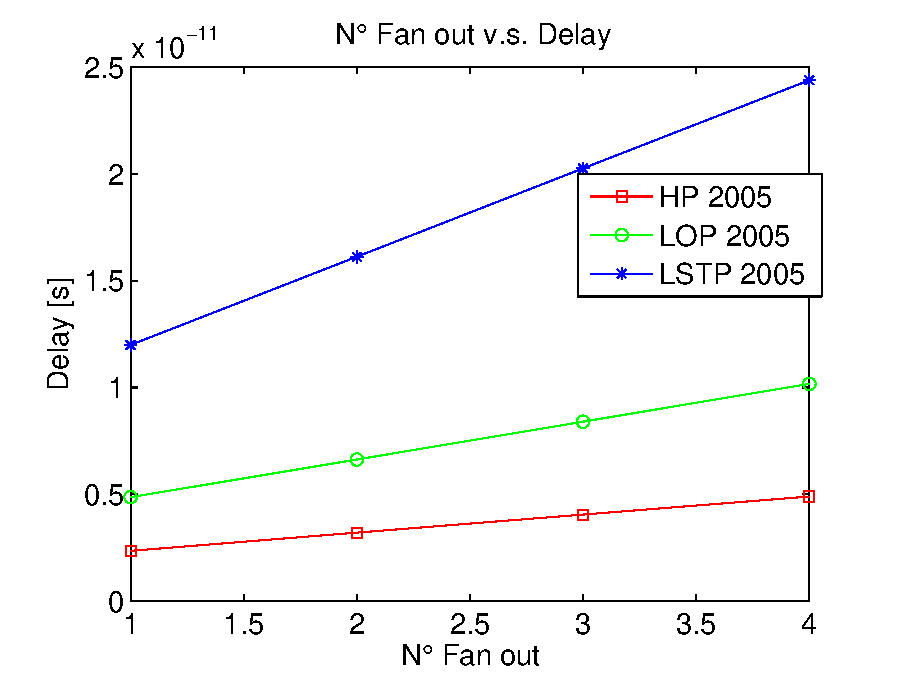
\includegraphics[width=0.8\textwidth]{img/plot_fanout_delay.eps}
\caption{Fan-out vs delay}
\label{fig:fan-out_plot}
\end{center}
\end{figure}
As we expected, increasing the fan-out, the delay increases too and find out also that HP technology has lower delay respect to LOP and LSTP, moreover its slope is less than other two. \\In figure \ref{fig:vdd_plot} is shown the delay variations for different $V_{DD}$ values according the three technology families.
\begin{figure}[htbp]
\begin{center}
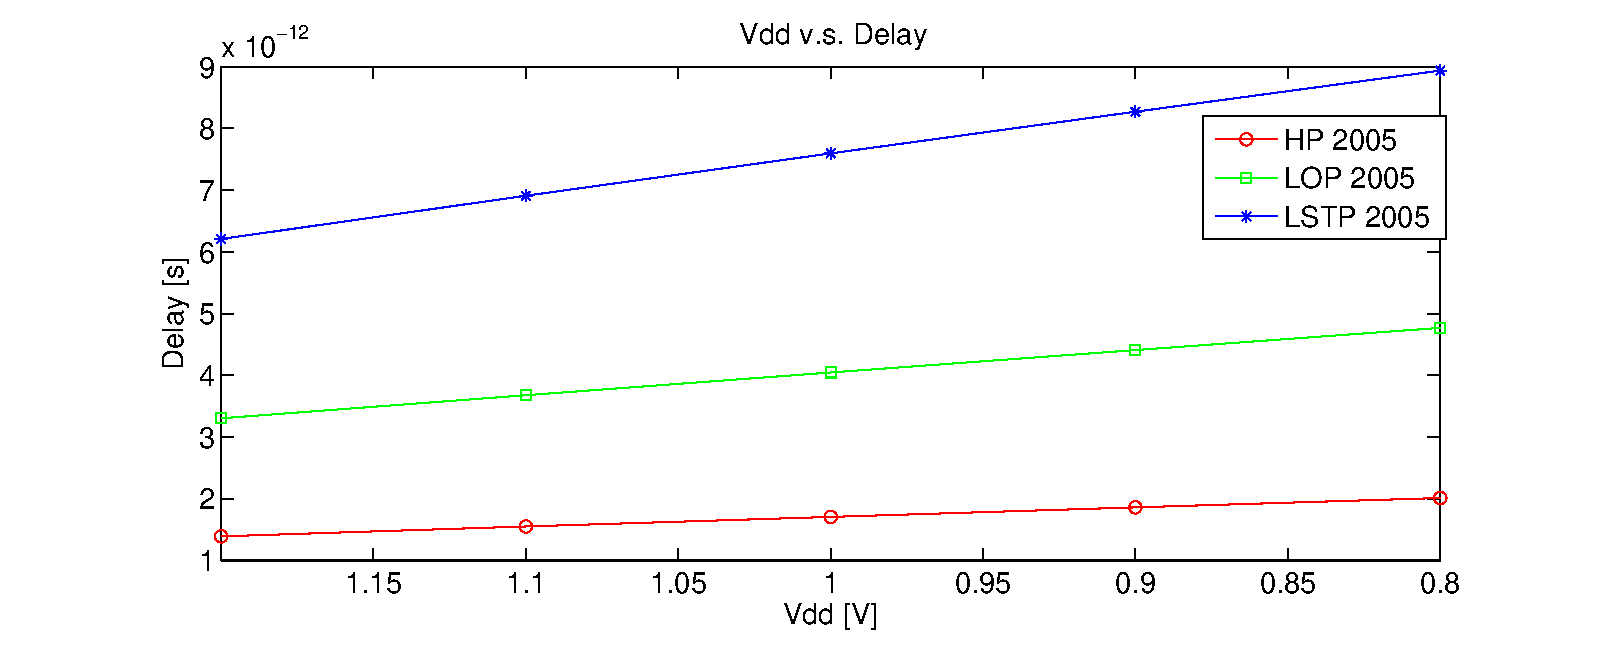
\includegraphics[width=0.8\textwidth]{img/plot_vdd_delay.eps}
\caption{$V_{DD}$ vs delay}
\label{fig:vdd_plot}
\end{center}
\end{figure}
As we expected, delay increases as $V_{dd}$ decreases. As before, the slope of HP is lower than the other two but less compared to fan-out plot. \\About power, in table \ref{tab:power} are reported static and dynamic power for the three families at 2005.
\vspace{2cm}
\\
\textbf{NOTE:} Variable Cox received in input at our module should be in $pF/\mu m^2$, but we have verified that must be multiplied by 10 to have a correct Cox.
\begin{table}[htdp]
\begin{center}
\begin{tabular}{|c|c|c|c|}
\hline
 & HP [W] & LOP [W] & LSTP [W]\\
\hline
P static & $3.7411\cdotp 10^{-4}$ & $2.3884\cdotp 10^{-6}$ & $1.6137\cdotp 10^{-8}$\\
\hline
P dynamic & $2.518\cdotp 10^{-6}$ & $1.3937\cdotp 10^{-6}$ & $2.4310\cdotp 10^{-6}$\\
\hline
\end{tabular}
\end{center}
\caption{Static and dynamic power for 2005 technological node}
\label{tab:power}
\end{table}

\newpage
%%%% this is an example
%\bibitem[topic]{label} Surname, Name, \emph{Title}, Editor, Location, Date, etc.

\begin{thebibliography}{report\_nand}
\bibitem{elmore_example1} N.H.E. Weste and D. Harris, \emph{"CMOS VLSI design, A circuits and systems perspective"}
\bibitem{elmore_example2} Rabaey, Chandrakasan and Nikolic, \emph{"Digital integrated circuits, a design perspective"}
\end{thebibliography}

\end{document}

